\documentclass{beamer}

\usepackage[utf8]{inputenc}
\usepackage{adjustbox}
\usepackage[T2A]{fontenc}
\usepackage{amssymb}
\usepackage{amsmath}
\usepackage{mathrsfs}
\usepackage{euscript}
\usepackage{upgreek}
\usepackage[english,russian]{babel}
\usepackage{array}
\usepackage{theorem}
\usepackage[all]{xy}
\usepackage{subfig}
\usepackage{epstopdf}   
\usepackage{tikz}       
\usepackage{pgfplots}   
\usepackage{color}
\usepackage{ifthen}
\usepackage{url}
\usepackage{makeidx}
\usepackage{pb-diagram}
\usepackage{balance}
\usepackage{multirow} 
\usepackage{bibentry}
\usepackage{booktabs}
\usepackage{cmap}
\usepackage{amsthm}
\usepackage[linesnumbered,ruled,vlined]{algorithm2e}
\usepackage[absolute]{textpos}
\usepackage{fleqn,psfrag,wrapfig,tikz}
\usepackage{algpseudocode}
\usepackage{amsmath}

\usepackage{graphics}
\usepackage{graphicx} % Allows including images
\usepackage{tabularx}
%\usepackage{jmlda}
\usetheme{Warsaw}
\usecolortheme{sidebartab}
%\definecolor{beamer@blendedblue}{RGB}{15,80,120}
\DeclareMathOperator*{\argmax}{arg\,max}
%----------------------------------------------------------------------------------------------------------
\title[\hbox to 56mm{Достаточный объем выборки  \hfill\insertframenumber\,/\,\inserttotalframenumber}]
{Раннее прогнозирование достаточного объема выборки для обобщенной линейной модели}
\author[В.\,С.~Бучнев]{Валентин Бучнев}
\institute{Московский физико-технический институт}
\date{\footnotesize{
\par\emph{Курс:} Численные методы обучения по прецедентам
(практика, В. В. Стрижов), группа 694, весна 2019
\par\emph{консультант:} А.\,В.~Грабовой
\date{qq}
}}



\begin{document}

\begin{frame}
\titlepage % Print the title page as the first slide
\end{frame}

\begin{frame}
\frametitle{Прогнозирование объема выборки}
\begin{block}{Цель исследования}
Предложить метод предсказания достаточного объема выборки для обобщенной линейной модели на ранних этапах сбора данных.
\end{block}
\begin{block}{Проблема}
Большинство неассимптотических методов требуют заведомо избыточного объема выборки.
\end{block}
\begin{block}{Метод решения}
Оценка объема строится по собранной выборке путем анализа свойств функции ошибки обобщенной линейной модели.
\end{block}

\end{frame}

\begin{frame}
\frametitle{Существующие методы}

\textbf{Ассимптотические методы}

\begin{itemize}
  \item S.\,G.\;Self and R.\,H.,\; Mauritsen Power/sample size calculations for generalized linear
models~//~Biometrics, 1988
  \item G.\,Shieh,\;On power and sample size calculations for likelihood ratio tests in generalized linear models~//~Biometrics, 2000.
  \item G.\,Shieh\;On power and sample size calculations for Wald tests in generalized linear models~//~Journal of Statistical Planning and Inference, 2005.
\end{itemize}

\textbf{Байесовские методы}

\begin{itemize}
  \item D.\,B.\;Rubin and H.\,S.\;Stern\;Sample size determination using posterior predictive distributions~//~Sankhya : The Indian Journal of Statistics Special Issue on Bayesian Analysis, 1998.
\end{itemize}

\end{frame}

\begin{frame}
\frametitle{Постановка задачи раннего прогнозирования}
\begin{block}{Дано}
Выборка размера m: $~\mathfrak D_m = \{\textbf{x}_i, y_i\}_{i=1}^m,$

где $\textbf{x}_i \in \mathbb{R}^{n}$ - вектор признаков, $~y_i \in \mathbb{Y}$.
\end{block}
\begin{block}{Функция правдоподобия}
Определим функцию правдоподобия и логарифмическую функцию правдоподобия выборки $\mathfrak D$:
$$
L(\mathfrak D_m, \textbf{w}) = \prod_{y, \textbf{x} \in \mathfrak D_m} f(y, \textbf{x}, \textbf{w}),~~~ l(\mathfrak D_m, \textbf w) = \sum_{y, \textbf{x} \in \mathfrak D_m}\log f(y, \textbf{x}, \textbf{w}),
$$
где $f(y, \textbf{x}, \textbf{w})$ - аппроксимация плотности апостериорной вероятности выборки $\mathfrak D_m$ при заданном векторе параметров $\textbf{w}$.
\end{block}
\end{frame}

\begin{frame}
\frametitle{Постановка задачи раннего прогнозирования}
\begin{block}{Логарифмическая функция правдоподобия}
Будем рассматривать ожидаемое значение функции $l$:

$$
\tilde{l}(\mathfrak D)  = \underset{y, \textbf{x} \in \mathfrak D}{\mathsf E} l(\{y, \textbf{x}\}, \textbf w).
$$
\end{block}
\begin{block}{Ожидаемое значение}
Рассмотрим ожидаемое значение логарифма правдоподобия по разным обучающим выборкам $\mathfrak D_{\mathcal L_m}$ размера $m^*$:

$$
l(m^*) = \underset{\mathfrak D_{\mathcal L_m}}{\mathsf E} \tilde{l}(\mathfrak D_{\mathcal L_m}).
$$
\end{block}
\end{frame}


\begin{frame}
\frametitle{Постановка задачи раннего прогнозирования}
\begin{block}{Критерий достаточности объема}
Будем считать, что объем выборки достаточный, если:

$$
\forall m_1, m_2 > m^* ~~~ |l(m_1) - l(m_2)| < \varepsilon,
$$
где $\varepsilon$ - достаточно малое пороговое значение.
\end{block}
\end{frame}

\begin{frame}
\frametitle{Предлагаемый метод решения}

\begin{block}{Критерий средней длины}
$$
A(\mathfrak{D}) = \{\textbf{w} : ||\textbf{w}- \hat{\textbf{w}}|| \leqslant r_m\}
$$
$$
\mathsf{P}(A(\mathfrak{D})) = 1 - \alpha,
$$
где $\alpha$ --- некоторое малое значение. 

Критерий средней длины выглядит следующим образом:

$$
\forall m \geqslant m^{*}~\mathsf{E}_{\mathfrak D_m} r_m \leqslant l , 
$$
где $r_m$ --- радиус шара $A(\mathfrak{D}_m)$, $l$ --- некоторое наперед заданное достаточно малое значение.
\end{block}
\end{frame}

\begin{frame}
\frametitle{Модификация критерия средней длины}

\begin{block}{Оценка вектора параметров}
Для оценки вектора параметров используется принцип максимума правдоподобия:
$$
\hat{\textbf{w}} = \argmax_{\textbf{w} \in \mathbb{W}} L(\mathfrak D_{\mathcal L_m}, \textbf{w}).
$$
\end{block}


\begin{block}{Вычисление функции эффективности}
Воспользуемся несмещеностью и состоятельностью оценки $\hat{\textbf{w}}$:

$$
\mathsf{E}\hat{\textbf{w}} = \textbf{m}, ~~~\mathsf{D}\hat{\textbf{w}} = \textbf{I}^{-1}(\mathfrak D_m),
$$
где $\textbf{I}(\mathfrak D_m)$ --- информационная матрица Фишера.
\end{block}
\end{frame}

\begin{frame}
\frametitle{Вычислительный эксперимент}
\begin{block}{Цель эксперимента}
Проверить работоспособность предложенного метода.
\end{block}

$\newline$

\textbf{Выборки из UCI репозитория.}

\begin{table}[h!]
\begin{center}
\label{table2}
\begin{tabularx}{\textwidth}{|p{1in}|X|X|c|}
\hline
	\centering Выборка &\centeringТип задачи&\centering Размер выборки& Число признаков\\
	\hline
	Servo &регрессия&\centering167&4\\
	\hline
	Boston &регрессия&\centering506&13\\
	\hline
	Diabetes&регрессия&\centering 442&5\\
\hline
\end{tabularx}
\end{center}
\end{table}
\end{frame}

\begin{frame}
\frametitle{Результаты}
\begin{figure}[h!t]\center
\subfloat{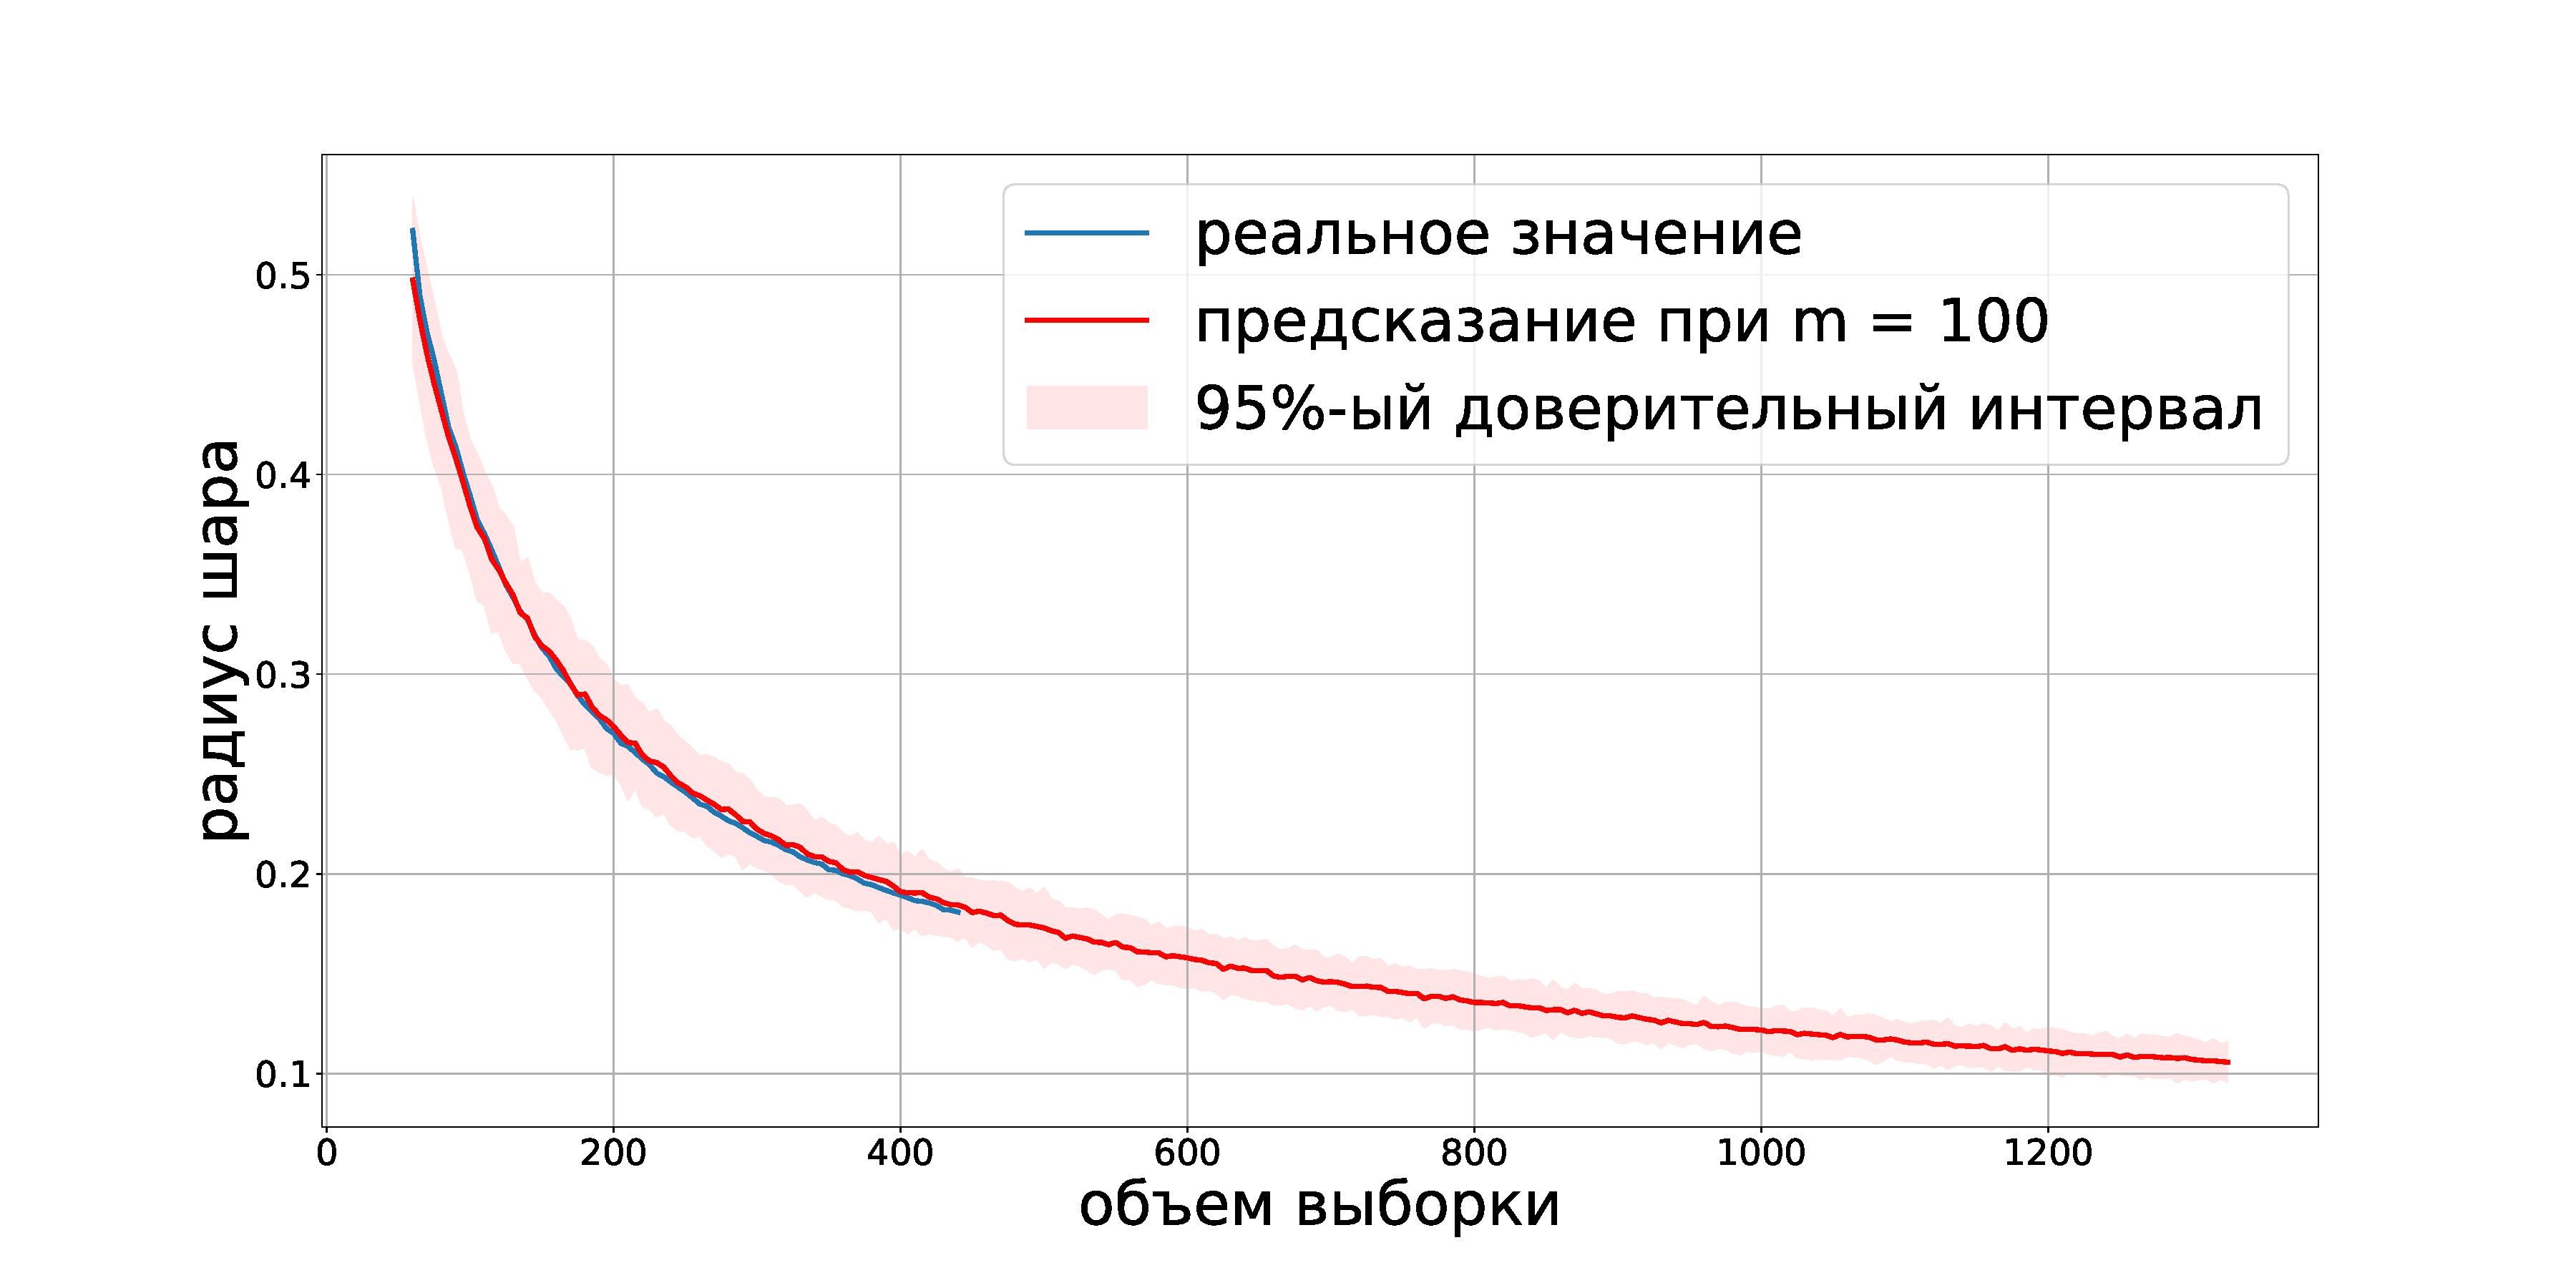
\includegraphics[width=1\textwidth]{../data/pics/ALC_modified_diabetes.pdf}}\\

\caption{ALC метод, выборка Diabetes}
\label{fig1}
\end{figure}
\end{frame}

\begin{frame}
\frametitle{Результаты}


\textbf{Предсказание достаточного объема выборки, ALC метод.}
\begin{table}[h]
\label{table2}
\begin{tabularx}{0.7\textwidth}{|p{1in}|X|c|}
\hline
	\centering Выборка & \centering Реальное значение &Предсказание\\
	\hline
	 Servo & \centering не хватает данных & 450\\
	\hline
	Boston & \centering не хватает данных &1370\\
	\hline
	Diabetes & \centering 235 & 240\\
\hline
\end{tabularx}
\end{table}

\end{frame}

\begin{frame}
\frametitle{Заключение}

\begin{itemize}
  \item Задача прогнозирования достаточного объема выборки сведена к задаче аппроксимации корреляционной матрицы вектора параметров.
  \item Показана работоспособность предложенного метода на тестовых выборках.
  \item Далее предлагается строить аппроксимацию зависимости ожидаемого значения логарифма правдоподобия от размера выборки.
\end{itemize}

\end{frame}


\end{document}